%%%%%%%%%%%%%%%%%%%%%%%%%%%%%%%%%%%%%%%%%%%%%%%%%%%%%%%%%%%%%%%%%%%%%%%%
%
%   SMT-COMP 2021 - Presentation on SMT-Workshop
%                   virtual conference in "Los Angeles"
%
%   1 hour
%
%%%%%%%%%%%%%%%%%%%%%%%%%%%%%%%%%%%%%%%%%%%%%%%%%%%%%%%%%%%%%%%%%%%%%%%%

\documentclass[table]{beamer}
\usepackage[utf8]{inputenc}
\usepackage{xcolor}
\usepackage{tikz}
\usetikzlibrary{shapes,shapes.callouts,automata,trees}
\usetikzlibrary{decorations.pathmorphing,external,fit}
\usetikzlibrary{calc}
\usetikzlibrary{backgrounds} %used for the CEGAR figure
\usepackage{amssymb}
\usepackage{clrscode}
\usepackage{pifont}
\usepackage{pdfpages}
\geometry{papersize={16cm,9cm}}
%\tikzexternalize

\colorlet{MYred}{red!70!black}
\definecolor{MYgreen}{rgb}{.1,.5,0}
\definecolor{MYblue}{rgb}{0,.42,.714}
\colorlet{MYgray}{white!95!MYblue}
\colorlet{MYorange}{orange!80!black}
\definecolor{gold}{rgb}{.8,.6,0}
\colorlet{silver}{white!55!black}
\colorlet{bronze}{brown!70!black}
\def\tick{\ding{52}}
\def\cross{\ding{54}}

%%%%%%%%%%%%%%%%%%%%
%%% Beamer stuff %%%
%%%%%%%%%%%%%%%%%%%%
\usetheme{default}
\useinnertheme{rounded}
\setbeamertemplate{frametitle}[default][center]
\setbeamertemplate{footline}{\quad\hfill\footnotesize\insertframenumber\strut\kern1em\vskip2pt}
\setbeamertemplate{navigation symbols}{}
\setbeamertemplate{itemize/enumerate subbody begin}{\normalsize}
\usefonttheme[onlymath]{serif} % Nicer formulas
\setbeamercolor{block body}{bg=black!10}
\setbeamercolor{block title}{bg=black!20}

\AtBeginSection[]{
  \begin{frame}
  \vfill
  \centering
  \begin{beamercolorbox}[sep=8pt,center,shadow=true,rounded=true]{title}
    \usebeamerfont{title}\insertsectionhead\par%
  \end{beamercolorbox}
  \vfill
  \end{frame}
}

\def\emph#1{\textcolor{MYblue}{#1}}

%%% Titel, Autor und Datum des Vortrags:
\title{SMT-COMP 2021\\
16th International Satisfiability Modulo Theory Competition}
\author{Haniel Barbosa \and \emph{Jochen Hoenicke} \and Antti Hyv\"arinen}
\date{July 18, 2021}

%% Institut
\institute{
  Universidade Federal de Minas Gerais, Brazil \and
  Albert-Ludwigs-Universit\"at Freiburg, Germany \and
  Universita della Svizzera italiana, Switzerland
}


%%%%%%%%%%%%%%%%%%%%%%%%%%%%%%%
% MACROS

% database symbol (from stackexchange)

\makeatletter
\tikzset{
    database/.style={
        path picture={
            \draw (0, 1.5*\database@segmentheight) circle [x radius=\database@radius,y radius=\database@aspectratio*\database@radius];
            \draw (-\database@radius, 0.5*\database@segmentheight) arc [start angle=180,end angle=360,x radius=\database@radius, y radius=\database@aspectratio*\database@radius];
            \draw (-\database@radius,-0.5*\database@segmentheight) arc [start angle=180,end angle=360,x radius=\database@radius, y radius=\database@aspectratio*\database@radius];
            \draw (-\database@radius,1.5*\database@segmentheight) -- ++(0,-3*\database@segmentheight) arc [start angle=180,end angle=360,x radius=\database@radius, y radius=\database@aspectratio*\database@radius] -- ++(0,3*\database@segmentheight);
        },
        minimum width=2*\database@radius + \pgflinewidth,
        minimum height=3*\database@segmentheight + 2*\database@aspectratio*\database@radius + \pgflinewidth,
    },
    database segment height/.store in=\database@segmentheight,
    database radius/.store in=\database@radius,
    database aspect ratio/.store in=\database@aspectratio,
    database segment height=0.1cm,
    database radius=0.25cm,
    database aspect ratio=0.35,
}
\makeatother


%%%%%%%%%%%%%%%%%%%%%%%%%%%%%%%

\begin{document}

\begin{frame}
  \titlepage
\end{frame}


\begin{frame}
  \frametitle{SMT-COMP}

  \begin{minipage}[b]{.6\textwidth}
    Annual competition for \emph{SMT solvers}\\
    on (a selection of) benchmarks from \emph{SMT-LIB}
  \end{minipage}%
  \begin{minipage}{.4\textwidth}
    \begin{block}{History}
      \begin{tabular}{rp{3cm}}
        \textbf{2005} & first competition \\
        \textbf{2013} & evaluation instead \\
        & of competition\\
        \textbf{2014} & since then hosted\\
        & by \emph{StarExec}\\
        \textbf{2021} & 16th competition
      \end{tabular}
    \end{block}
  \end{minipage}

  Goals:
  \begin{itemize}
  \item spur development of SMT solver implementations
  \item promote SMT solvers and their usage
  \item support the SMT-LIB project
    \begin{itemize}
    \item to promote and develop the SMT-LIB format
    \item to collect relevant benchmarks
    \end{itemize}
  \item engage and include new members
  \end{itemize}

\end{frame}



\begin{frame}
  \frametitle{SMT Solvers and SMT-LIB}
  SMT Solver
  \begin{itemize}
  \item checks formulas 
    in \emph{SMT-LIB} format
    for \emph{satisfiability modulo theories}
  \end{itemize}
  \bigskip

  SMT-LIB is
  \begin{enumerate}
  \item a \emph{language} in which benchmarks are written
  \item a community effort to \emph{collect benchmarks}
  \end{enumerate}
  \medskip

  \begin{columns}
    \begin{column}{0.4\textwidth}
      \begin{block}{Non-incremental}
        381\,683 instances {\small (+5082)} \\
        with 1 query each \\
        in 79 logics {\small (+9)}.
      \end{block}
    \end{column}
    \begin{column}{0.4\textwidth}
      \begin{block}{Incremental}
        43\,284 instances {\small (+19\,073)}\\
        with 33\,998\,794 queries {\small (+554\,499)} \\
        in 35 logics {\small (+2)}.
      \end{block}
    \end{column}
    \begin{column}{0.08\textwidth}
    \end{column}
  \end{columns}
\end{frame}

\begin{frame}
  \frametitle{SMT-LIB Logics}

  
  \noindent\makebox[\textwidth]{%
  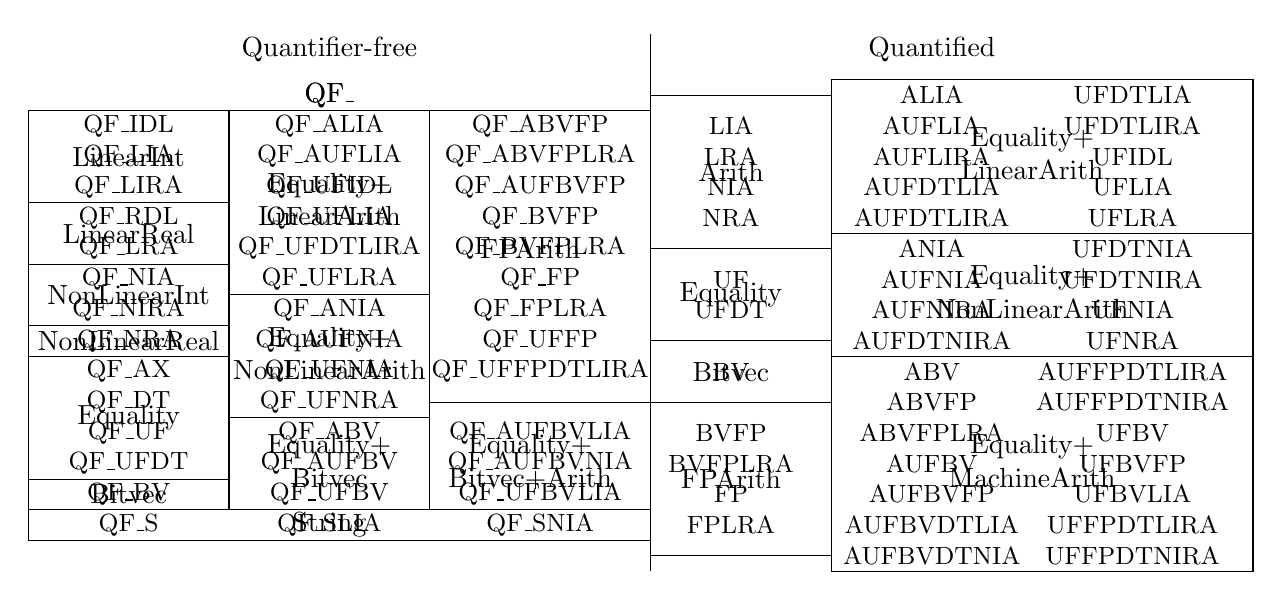
\begin{tikzpicture}[xscale=2.55,yscale=.39]
    \uncover<1-3> {
    % Arith
    \node at (3,14) {\small LIA};
    \node at (3,13) {\small LRA};
    \node at (3,12) {\small NIA};
    \node at (3,11) {\small NRA};
    % Equality
    \node at (3,9) {\small UF};
    \node at (3,8) {\small UFDT};
    % Bitvec
    \node at (3,6) {\small BV};
    % FPArith
    \node at (3,4) {\small BVFP};
    \node at (3,3) {\small BVFPLRA};
    \node at (3,2) {\small FP};
    \node at (3,1) {\small FPLRA};
    % Equality+LinearArith
    \node at (4,15) {\small ALIA};
    \node at (4,14) {\small AUFLIA};
    \node at (4,13) {\small AUFLIRA};
    \node at (4,12) {\small AUFDTLIA};
    \node at (4,11) {\small AUFDTLIRA};
    \node at (5,15) {\small UFDTLIA};
    \node at (5,14) {\small UFDTLIRA};
    \node at (5,13) {\small UFIDL};
    \node at (5,12) {\small UFLIA};
    \node at (5,11) {\small UFLRA};
    % Equality+NonLinearArith
    \node at (4,10) {\small ANIA};
    \node at (4,9) {\small AUFNIA};
    \node at (4,8) {\small AUFNIRA};
    \node at (4,7) {\small AUFDTNIRA};
    \node at (5,10) {\small UFDTNIA};
    \node at (5,9) {\small UFDTNIRA};
    \node at (5,8) {\small UFNIA};
    \node at (5,7) {\small UFNRA};
    % Equality+MachinedArith
    \node at (4,6) {\small ABV};
    \node at (4,5) {\small ABVFP};
    \node at (4,4) {\small ABVFPLRA};
    \node at (4,3) {\small AUFBV};
    \node at (4,2) {\small AUFBVFP};
    \node at (4,1) {\small AUFBVDTLIA};
    \node at (4,0) {\small AUFBVDTNIA};
    \node at (5,6) {\small AUFFPDTLIRA};
    \node at (5,5) {\small AUFFPDTNIRA};
    \node at (5,4) {\small UFBV};
    \node at (5,3) {\small UFBVFP};
    \node at (5,2) {\small UFBVLIA};
    \node at (5,1) {\small UFFPDTLIRA};
    \node at (5,0) {\small UFFPDTNIRA};

    %QF_LinearIntArith
    \node at (0,14) {\small QF\_IDL};
    \node at (0,13) {\small QF\_LIA};
    \node at (0,12) {\small QF\_LIRA};
    %QF_LinearRealArith
    \node at (0,11) {\small QF\_RDL};
    \node at (0,10) {\small QF\_LRA};
    %QF_NonLinearIntArith
    \node at (0,9) {\small QF\_NIA};
    \node at (0,8) {\small QF\_NIRA};
    %QF_NonLinearRealArith
    \node at (0,7) {\small QF\_NRA};
    %QF_Equality
    \node at (0,6) {\small QF\_AX};
    \node at (0,5) {\small QF\_DT};
    \node at (0,4) {\small QF\_UF};
    \node at (0,3) {\small QF\_UFDT};
    %QF_Bitvec
    \node at (0,2) {\small QF\_BV};
    %QF_Strings
    \node at (0,1) {\small QF\_S};
    \node at (1,1) {\small QF\_SLIA};
    \node at (2.05,1) {\small QF\_SNIA};
    %QF_Equality+LinearArith
    \node at (1,14) {\small QF\_ALIA};
    \node at (1,13) {\small QF\_AUFLIA};
    \node at (1,12) {\small QF\_UFIDL};
    \node at (1,11) {\small QF\_UFLIA};
    \node at (1,10) {\small QF\_UFDTLIRA};
    \node at (1,9) {\small QF\_UFLRA};
    %QF_Equality+NonLinearArith
    \node at (1,8) {\small QF\_ANIA};
    \node at (1,7) {\small QF\_AUFNIA};
    \node at (1,6) {\small QF\_UFNIA};
    \node at (1,5) {\small QF\_UFNRA};
    %QF_Equality+Bitvec
    \node at (1,4) {\small QF\_ABV};
    \node at (1,3) {\small QF\_AUFBV};
    \node at (1,2) {\small QF\_UFBV};
    %QF_Equality+Bitvec+Arith
    \node at (2.05,4) {\small QF\_AUFBVLIA};
    \node at (2.05,3) {\small QF\_AUFBVNIA};
    \node at (2.05,2) {\small QF\_UFBVLIA};
    %QF_FPArith
    \node at (2.05,14) {\small QF\_ABVFP};
    \node at (2.05,13) {\small QF\_ABVFPLRA};
    \node at (2.05,12) {\small QF\_AUFBVFP};
    \node at (2.05,11) {\small QF\_BVFP};
    \node at (2.05,10) {\small QF\_BVFPLRA};
    \node at (2.05,9) {\small QF\_FP};
    \node at (2.05,8) {\small QF\_FPLRA};
    \node at (2.05,7) {\small QF\_UFFP};
    \node at (2.05,6) {\small QF\_UFFPDTLIRA};
    }
    %
    \uncover<2-> {
      \draw (2.6,-0.5) -- (2.6,17);
      \node at (1,16.5) {Quantifier-free};
      \node at (4,16.5) {Quantified};
    }
    \uncover<3-> {
      \draw (-.5,.5) rectangle (2.6,1.5);
      \draw (-.5,1.5) rectangle (.5,2.5);
      \draw (-.5,2.5) rectangle (.5,6.5);
      \draw (-.5,6.5) rectangle (.5,7.5);
      \draw (-.5,7.5) rectangle (.5,9.5);
      \draw (-.5,9.5) rectangle (.5,11.5);
      \draw (-.5,11.5) rectangle (.5,14.5);
      \draw (.5,1.5) rectangle (1.5,4.5);
      \draw (.5,4.5) rectangle (1.5,8.5);
      \draw (.5,8.5) rectangle (1.5,14.5);
      \draw (1.5,1.5) rectangle (2.6,5);
      \draw (1.5,5) rectangle (2.6,14.5);
      
      \draw (2.6,0) rectangle (3.5,5);
      \draw (2.6,5) rectangle (3.5,7);
      \draw (2.6,7) rectangle (3.5,10);
      \draw (2.6,10) rectangle (3.5,15);
      \draw (3.5,-.5) rectangle (5.6,6.5);
      \draw (3.5,6.5) rectangle (5.6,10.5);
      \draw (3.5,10.5) rectangle (5.6,15.5);
    }
    \uncover<4-> {
      \node at (1,15) {QF\_};
      \node at (0,13) {LinearInt};
      \node at (0,10.5) {LinearReal};
      \node at (0,8.5) {NonLinearInt};
      \node at (0,7) {NonLinearReal};
      \node at (0,4.5) {Equality};
      \node at (0,2) {Bitvec};
      \node at (1,11.5) {\begin{tabular}{c}Equality+\\LinearArith\end{tabular}};
      \node at (1,6.5) {\begin{tabular}{c}Equality+\\NonLinearArith\end{tabular}};
      \node at (1,3) {\begin{tabular}{c}Equality+\\Bitvec\end{tabular}};
      \node at (1,1) {String};
      \node at (2,10) {FPArith};
      \node at (2,3) {\begin{tabular}{c}Equality+\\Bitvec+Arith\end{tabular}};
      \node at (1,15) {QF\_};
      
      \node at (3,12.5) {Arith};
      \node at (3,8.5) {Equality};
      \node at (3,6) {Bitvec};
      \node at (3,2.5) {FPArith};

      \node at (4.5,13) {\begin{tabular}{c}Equality+\\LinearArith\end{tabular}};
      \node at (4.5,8.5) {\begin{tabular}{c}Equality+\\NonLinearArith\end{tabular}};
      \node at (4.5,3){\begin{tabular}{c}Equality+\\MachineArith\end{tabular}};
    }
  \end{tikzpicture}
  }

  \uncover<2-3>{
    \small
    \textbf{Q}uantifier \textbf{F}ree
    \textbf{A}rray
    \textbf{U}ninterpreted \textbf{F}unction
    \textbf{B}it\textbf{V}ector
    \textbf{F}loating\textbf{P}oint
    \textbf{D}ata\textbf{T}ype
    \textbf{S}trings
    \textbf{N}onlinear/\textbf{L}inear
    \textbf{I}nteger \textbf{R}eal
    \textbf{A}rithmetic
    \textbf{D}ifference \textbf{L}ogic
    }
\end{frame}


\begin{frame}
  \frametitle{Competition Overview}

  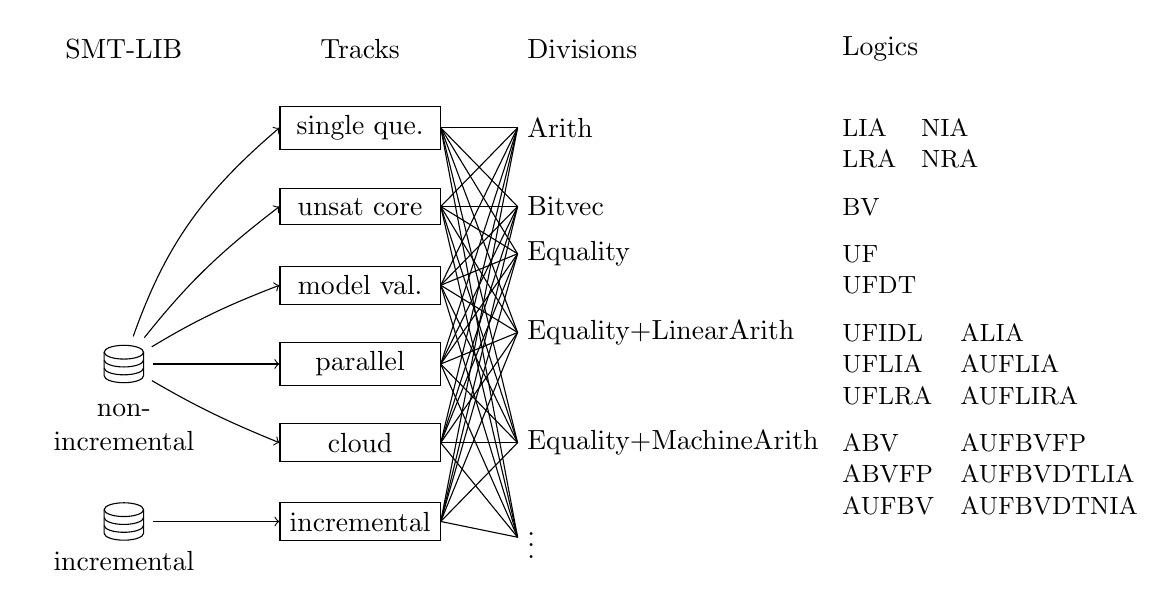
\begin{tikzpicture}
    \node at (0,6) {SMT-LIB};
    \node at (3,6) {Tracks};
    \node[anchor=west] at (5,6) {Divisions};
    \node[anchor=west] at (9,6) {Logics};
    
    \node[database,label=below:{\begin{tabular}{c}non-\\incremental\end{tabular}}] (nonincbench) at (0,2) {};
    \node[database,label=below:{incremental}] (incbench) at (0,0) {};

    \node[draw,text width=1.8cm,align=center](sq) at (3,5) {single que.};
    \node[draw,text width=1.8cm,align=center](uc) at (3,4) {unsat core};
    \node[draw,text width=1.8cm,align=center](mv) at (3,3) {model val.};
    \node[draw,text width=1.8cm,align=center](par) at (3,2) {parallel};
    \node[draw,text width=1.8cm,align=center](cloud) at (3,1) {cloud};
    \node[draw,text width=1.8cm,align=center](inc) at (3,0) {incremental};

    \node[anchor=west] (div1) at (5,5) {Arith};
    \node[anchor=west] at (9,5) {\small LIA};
    \node[anchor=west] at (9,4.6) {\small LRA};
    \node[anchor=west] at (10,5) {\small NIA};
    \node[anchor=west] at (10,4.6) {\small NRA};
    \node[anchor=west] (div2) at (5,4) {Bitvec};
    \node[anchor=west] at (9,4) {\small BV};
    \node[anchor=west] (div3) at (5,3.4) {Equality};
    \node[anchor=west] at (9,3.4) {\small UF};
    \node[anchor=west] at (9,3) {\small UFDT};
    \node[anchor=west] (div4) at (5,2.4) {Equality+LinearArith};
    \node[anchor=west] at (9,2.4) {\small UFIDL};
    \node[anchor=west] at (9,2) {\small UFLIA};
    \node[anchor=west] at (9,1.6) {\small UFLRA};
    \node[anchor=west] at (10.5,2.4) {\small ALIA};
    \node[anchor=west] at (10.5,2) {\small AUFLIA};
    \node[anchor=west] at (10.5,1.6) {\small AUFLIRA};
    \node[anchor=west] at (12.5,2) {$\hdots$};
    \node[anchor=west] (div5) at (5,1) {Equality+MachineArith};
    \node[anchor=west] at (9,1) {\small ABV};
    \node[anchor=west] at (9,.6) {\small ABVFP};
    \node[anchor=west] at (9,.2) {\small AUFBV};
    \node[anchor=west] at (10.5,1) {\small AUFBVFP};
    \node[anchor=west] at (10.5,.6) {\small AUFBVDTLIA};
    \node[anchor=west] at (10.5,.2) {\small AUFBVDTNIA};
    \node[anchor=west] at (12.5,1) {$\hdots$};
    \node[anchor=west] (div6)  at (5,-.2) {$\vdots$};

    \draw[->,shorten <=.3em] (nonincbench) to[bend left=15] (sq.west);
    \draw[->,shorten <=.3em] (nonincbench) to[bend left=7] (uc.west);
    \draw[->,shorten <=.3em] (nonincbench) to[bend left=5] (mv.west);
    \draw[->,shorten <=.3em] (nonincbench) to (par.west);
    \draw[->,shorten <=.3em] (nonincbench) to[bend right=4] (cloud.west);
    \draw[->,shorten <=.3em] (incbench) to (inc.west);

    \draw (sq.east) to (div1.west);
    \draw (sq.east) to (div2.west);
    \draw (sq.east) to (div3.west);
    \draw (sq.east) to (div4.west);
    \draw (sq.east) to (div5.west);
    \draw (sq.east) to (div6.west);

    \draw (uc.east) to (div1.west);
    \draw (uc.east) to (div2.west);
    \draw (uc.east) to (div3.west);
    \draw (uc.east) to (div4.west);
    \draw (uc.east) to (div5.west);
    \draw (uc.east) to (div6.west);

    \draw (mv.east) to (div1.west);
    \draw (mv.east) to (div2.west);
    \draw (mv.east) to (div3.west);
    \draw (mv.east) to (div4.west);
    \draw (mv.east) to (div5.west);
    \draw (mv.east) to (div6.west);

    \draw (cloud.east) to (div1.west);
    \draw (cloud.east) to (div2.west);
    \draw (cloud.east) to (div3.west);
    \draw (cloud.east) to (div4.west);
    \draw (cloud.east) to (div5.west);
    \draw (cloud.east) to (div6.west);

    \draw (par.east) to (div1.west);
    \draw (par.east) to (div2.west);
    \draw (par.east) to (div3.west);
    \draw (par.east) to (div4.west);
    \draw (par.east) to (div5.west);
    \draw (par.east) to (div6.west);

    \draw (inc.east) to (div1.west);
    \draw (inc.east) to (div2.west);
    \draw (inc.east) to (div3.west);
    \draw (inc.east) to (div4.west);
    \draw (inc.east) to (div5.west);
    \draw (inc.east) to (div6.west);
  \end{tikzpicture}

\end{frame}

\begin{frame}[fragile]{SMT-COMP Tracks (traditional)}
  \emph{Single Query Track}
  \begin{itemize}
  \item Determine satisfiability of one problem
  \item Solver answers sat/unsat/unknown
  \end{itemize}
  \medskip

  \emph{Unsat Core Track}
  \begin{itemize}
  \item Find small unsatisfiable subset of input.
  \item Solver answers unsat + list of formulas.
  \end{itemize}
  \medskip
 
  \emph{Model Validation Track}
  \begin{itemize}
  \item Find a model for a satisfiable problem.
  \item Solver answers sat + value for each non-logical symbol.
  \end{itemize}
  \medskip

  \emph{Incremental Track}
  \begin{itemize}
  \item Solve many small problems interactively.
  \item Solver acks commands and answers sat/unsat for each check.
  \end{itemize}
\end{frame}

\begin{frame}[fragile]{SMT-COMP Tracks (new)}
  SMT-COMP 2021 has two new experimental tracks (sponsored by AWS).
  \bigskip
  
  \emph{Parallel Track}
  \begin{itemize}
  \item Solve a large problem on a big computer
    \begin{itemize}
    \item 64 cores, 256 GB of memory
    \end{itemize}
  \item Solver answers sat/unsat/unknown
  \end{itemize}
  \bigskip
  \emph{Cloud Track}
  \begin{itemize}
  \item Solve a large problem on a network of computers
    \begin{itemize}
    \item 100 machines, 1600 cores, 6400 GB of memory
    \end{itemize}
  \item Solver answers sat/unsat/unknown
  \end{itemize}
\end{frame}


\begin{frame}{Tracks, Solvers, Divisions, and Benchmarks}
  Teams: 18 (+2)
  \bigskip

  \begin{tabular}{c|r@{}l|r@{}l|c}
    Track & \multicolumn{2}{c|}{Solvers} & \multicolumn{2}{c|}{Divisions}  & Benchmarks \\
    \hline
    Single Query  &  19&(-1)  & 18&(-49)  & 101300/381683 \\
    Incremental &  7&(-2)   & 15&(-11)  & 22233/43284   \\
    Unsat Core  &  7&(+2)   & 17&(-23)  & 55463/108188  \\
    Model Validation  &  7&(=)    &  3&(+2) + 3 exp.  & 13301/21251  \\
    Parallel &   &3      &   &14 exp.  & 413/20705 \\
    Cloud & &5      &   &14 exp.  & 405/20669 \\
  \end{tabular}
  \bigskip

  Number in parenthesis shows changes from 2020
\end{frame}

\begin{frame}
  \frametitle{Participants}

  SMT-COMP 2021 participants:
  \begin{itemize}
  \item classic CDCL(T)-based SMT solvers
  \item mcSAT-based solvers
  \item automated theorem provers
  \item finite domain solver
  \item local search techniques
  \item wrapper extending the scope of existing solvers
  \end{itemize}

  \bigskip
  Four new solvers participated:
  \begin{itemize}
  \item iProver (Konstantin Korovin, Andre Duarte, Edvard K Holden)
  \item mc2 (Simon Cruanes, Guillaume Bury)
  \item YicesLS (Bohan Li, Shaowei Cai, Xindi Zhang)
  \item YicesQS (Stéphane Graham-Lengrand)
  \end{itemize}

\end{frame}




\section{Solver Presentation}


{
\begin{frame}
  \vspace*{-1pt}%
  \noindent\makebox[\textwidth]{%
    \includegraphics[height=\paperheight]{bitwuzla-nonumber.pdf}}
\end{frame}
}

{
\begin{frame}
  \vspace*{-1pt}%
  \noindent\makebox[\textwidth]{%
    \includegraphics[height=\paperheight]{COLIBRI-nonumber.pdf}}
\end{frame}
}

{
\begin{frame}
  \vspace*{-1pt}%
  \noindent\makebox[\textwidth]{%
    \includegraphics[height=\paperheight]{cvc5-nonumber.pdf}}
\end{frame}
}

{
\begin{frame}
  \vspace*{-1pt}%
  \noindent\makebox[\textwidth]{%
    \includegraphics[height=\paperheight]{cvc5-gg-nonumber.pdf}}
\end{frame}
}

{
\begin{frame}
  \vspace*{-1pt}%
  \noindent\makebox[\textwidth]{%
    \includegraphics[height=\paperheight]{iprover-nonumber.pdf}}
\end{frame}
}

{
\setbeamertemplate{footline}{\quad\hfill\footnotesize\textcolor{white}{\insertframenumber}\strut\kern1em\vskip1pt}
\begin{frame}
  \vspace*{-1pt}%
  \noindent\makebox[\textwidth]{%
    \includegraphics[height=\paperheight]{mc2-nonumber.pdf}}
\end{frame}
}


{
\begin{frame}
  \vspace*{-1pt}%
  \noindent\makebox[\textwidth]{%
    \includegraphics[height=\paperheight]{opensmt-nonumber.pdf}}
\end{frame}
}

{
\begin{frame}
  \vspace*{-1pt}%
  \noindent\makebox[\textwidth]{%
    \includegraphics[height=\paperheight]{smtinterpol-nonumber.pdf}}
\end{frame}
}

{
%\setbeamertemplate{footline}{\quad\hfill\footnotesize\textcolor{white}{\insertframenumber}\strut\kern1em\vskip1pt}
\begin{frame}<1,3>
  \vspace*{-1pt}%
  \noindent\makebox[\textwidth]{%
    \only<1>{%
      \includegraphics[height=\paperheight,page=1]{smt-rat-nonumber.pdf}
    }\only<2>{%
      \includegraphics[height=\paperheight,page=2]{smt-rat-nonumber.pdf}
    }\only<3>{%
      \includegraphics[height=\paperheight,page=3]{smt-rat-nonumber.pdf}
    }}%
\end{frame}
}

{
\begin{frame}
  \vspace*{-1pt}%
  \noindent\makebox[\textwidth]{%
    \includegraphics[height=\paperheight]{UltimateEliminator-nonumber.pdf}}
\end{frame}
}

{
\begin{frame}
  \vspace*{-1pt}%
  \noindent\makebox[\textwidth]{%
    \includegraphics[height=\paperheight]{vampire-nonumber.pdf}}
\end{frame}
}

{
\begin{frame}
  \vspace*{-1pt}%
  \noindent\makebox[\textwidth]{%
    \includegraphics[height=\paperheight]{verit-nonumber.pdf}}
\end{frame}
}


{
\begin{frame}
  \vspace*{-1pt}\vspace*{-.1\paperheight}%
  \noindent\makebox[\textwidth]{%
    \includegraphics[height=1.2\paperheight]{Yices-nonumber.pdf}}
\end{frame}
}

{
\begin{frame}
  \vspace*{-1pt}%
  \noindent\makebox[\textwidth]{%
    \includegraphics[height=\paperheight]{YicesQS-nonumber.pdf}}
\end{frame}
}

{
\begin{frame}
  \vspace*{-1pt}%
  \noindent\makebox[\textwidth]{%
    \includegraphics[height=\paperheight]{YicesLS-nonumber.pdf}}
\end{frame}
}

\begin{frame}
  \frametitle{Non-Competitive Solvers}

  Submitted by Organisers
  \begin{itemize}
  \item z3-4.8.11
  \item MathSAT 5.6.6
  \item Par4 (for Parallel Track)
  \item Division winners from last year (32 Solvers)
  \end{itemize}
  \bigskip

  Submitted by Participants
  \begin{itemize}
  \item Fixed solvers (Bitwuzla, COLIBRI, cvc5, iProver, OpenSMT, Vampire)
  \end{itemize}
\end{frame}

\begin{frame}
  \frametitle{New in 2021}

  \begin{itemize}
  \item model validation track extended
  \item manually checking and resolving disagreements
  \item multiple logics per division
  \item we will create an artifact
  \end{itemize}
\end{frame}


\begin{frame}[fragile]
  \frametitle{Model Validation Track}

  Solvers print model for each constant/uninterpreted function
\begin{verbatim}
sat
(model
  (define-fun x15 () Int 5)
  (define-fun x24 () x135 (as @1 x135))
  (define-fun x10 ((?X1 Int)) Int (ite (and (= ?X1 10)) 2 (ite...
\end{verbatim}

  \begin{itemize}
  \item model validator based on pySMT
  \item all models of the competitors were accepted
  \item validator is still inefficient ($>$ 15 minutes)
  \end{itemize}

  \bigskip

  Many thanks to \emph{Andrea Micheli}
\end{frame}

\begin{frame}{Checking Disagreements}

  \begin{itemize}
  \item 111285 instances of 381683 have no status
  \item we checked disagreements between solvers
  \item 209 non-incremental instances
    and 65 incremental instances
  \item only 28 had known sat/unsat status
  \item tactics to resolve status:
    \begin{itemize}
    \item similar disagreements on instances with known status
    \item confirmed with fixed version of participants
    \item analyzed model from solver claiming sat
    \item majority vote
    \item in rare cases manually analyzed instances
    \end{itemize}
  \item solvers found unsound: (Bitwuzla, COLIBRI, cvc5, iProver, MathSAT, OpenSMT, Par4, UltimateEliminator+MathSAT, Vampire, Z3str4)
  \end{itemize}
\end{frame}


\begin{frame}
  \frametitle{Divisions}
  Tracks are split into \emph{divisions}.

  \begin{itemize}
  \item \emph{before 2021}: Division = SMT-LIB logic
  \item \emph{2021}: 19 Divisions subdivided in 84 logics
  \end{itemize}

  This implied more changes:
  \begin{itemize}
  \item solver authors select supported logics
    \begin{itemize}
    \item[$\Rightarrow$] solvers may run on only a part of a division.
    \end{itemize}
  \item fewer winners (1--5 winners per division)
  \item two solvers won a logic but not a division
    \begin{itemize}
    \item YicesQS won NRA
    \item YicesLS won QF\_IDL
    \end{itemize}
  \end{itemize}
\end{frame}

\begin{frame}
  \frametitle{Statistics}
  Solver Size
  \begin{itemize}
  \item range from 930~kB to 196~MB (compressed)
  \item total 436 MB
  \item unsat core post-processor: 361~MB
  \end{itemize}
  \bigskip
  \pause
  
  Job statistics
  \begin{itemize}
  \item Total Job Size: $\sim$ 85 GB
    \begin{itemize}
    \item 35~GB YicesLS temporary files
    \item 29~GB z3 models
    \end{itemize}
  \item 1\,371\,593 pairs (+428\,000)
  \item 16.3 CPU years (+6.4), 9.22 computer years on StarExec
  \item excludes result processors, StarExec overhead, glitches
  \end{itemize}
\end{frame}


\begin{frame}{Scoring}
  Computing scores:
  \begin{itemize}
  \item \emph{Single Query/Parallel/Cloud}: number of solved \emph{instances}
  \item \emph{Incremental}: number of solved \emph{queries}
  \item \emph{Unsat Core}: number of top-level assertions \emph{removed}
  \item \emph{Model Validation}: number of solved instances with correct \emph{models}
  \end{itemize}

  \bigskip
  Error scores:
  \begin{itemize}
  \item \emph{All Tracks}: given for sat reply for unsat instance, or vice versa
  \item \emph{Unsat Core}: given if returned core is satisfiable.
  \item \emph{Model Validation}: given if given model evaluates formula to \emph{false}
  \end{itemize}
  Error scores are draconian.
\end{frame}

\begin{frame}{Score and Ranking}
  In each track we collect different scores:
  \begin{itemize}
  \item \emph{Sequential score} (SQ, UC, MV): all time limits apply to cpu time
  \item \emph{Parallel score} (all): all time limits apply to wallclock time
  \item \emph{SAT score} (SQ): parallel score for \emph{satisfiable} instances
  \item \emph{UNSAT score} (SQ): parallel score for \emph{unsatisfiable} instances
  \item \emph{24s} (SQ): parallel score with time limit of \emph{24s}
  \end{itemize}
  \bigskip

  Division ranking (for each score)
  \begin{itemize}
  \item For each division, one winner is declared
  \end{itemize}

  \bigskip

  Two competition-wide rankings (for each score)
  \begin{itemize}
  \item \emph{Biggest lead}: division winner with most score difference to second place
  \item \emph{Largest contribution}: improvement each solver provided to a virtual best solver
  \end{itemize}
  
\end{frame}

\begin{frame}{Division Winners}
  \pause
  \emph{Single Query}
  \begin{itemize}
  \item \emph{Bitwuzla}: {\small QF\_Bitvec, QF\_Equality+Bitvec}
  \item \emph{cvc5}: \begin{minipage}{.8\textwidth}\raggedright \tiny Arith, Bitvec, Equality, Equality+LinearArith, Equality+MachineArith, Equality+NonLinearArith, FPArith, QF\_Equality, QF\_Equality+LinearArith, QF\_Equality+NonLinearArith, QF\_FPArith, QF\_LinearIntArith, QF\_LinearRealArith, QF\_NonLinearIntArith, QF\_NonLinearRealArith, QF\_Strings\end{minipage}
  \item \emph{iProver}: {\small Equality+NonLinearArith}
  \item \emph{SMTInterpol}: {\small QF\_Equality+LinearArith}
  \item \emph{UltimateEliminator+MathSAT}: {\small Equality+NonLinearArith}
  \item \emph{Vampire}: {\small Arith, Equality, Equality+NonLinearArith}
  \item \emph{Yices2}: {\tiny QF\_Bitvec, QF\_Equality, QF\_LinearIntArith, QF\_LinearRealArith, QF\_NonLinearIntArith}
  \end{itemize}

  \medskip

  \pause
  \emph{Unsat Core}
  \begin{itemize}
  \item \emph{Bitwuzla}: {\small QF\_Bitvec, QF\_Equality+Bitvec, QF\_FPArith}
  \item \emph{cvc5}: \begin{minipage}{.8\textwidth}\raggedright \tiny Arith, Bitvec, Equality, Equality+LinearArith, Equality+MachineArith, Equality+NonLinearArith, FPArith, QF\_Equality, QF\_Equality+NonLinearArith, QF\_LinearIntrArith, QF\_NonLinearIntArith, QF\_NonLinearRealArith \end{minipage}
  \item \emph{Yices2}: {\small QF\_Equality+LinearArith, QF\_LinearRealArith}
  \end{itemize}

\end{frame}

\begin{frame}{Division Winners}
  \emph{Incremental}
  \begin{itemize}
  \item \emph{cvc5}: \begin{minipage}{.8\textwidth}\raggedright \tiny Arith, Bitvec, Equality, Equality+LinearArith, Equality+NonLinearArith, FPArith, QF\_Equality, QF\_Equality+LinearArith, QF\_FPArith\end{minipage}
  \item \emph{OpenSMT}: {\small QF\_LinearRealArith}
  \item \emph{SMTInterpol}: {\small QF\_Equality+NonLinearArith,QF\_NonLinearIntArith}
  \item \emph{STP}: {\small QF\_Bitvec}
  \item \emph{Yices2}: {\small QF\_Equality+Bitvec,QF\_LinearIntArith}
  \end{itemize}
  \medskip

  \pause
  \emph{Model Validation (competitive only)}
  \begin{itemize}
  \item \emph{Bitwuzla}: {\small QF\_Bitvec}
  \item \emph{cvc5}: {\small QF\_LinearIntArith}
  \item \emph{Yices2}: {\small QF\_LinearRealArith}
  \end{itemize}
\end{frame}

\begin{frame}{Largest contribution}
  \begin{tabular}{r|c@{}lc@{}lc@{}l}
    &\textcolor{gold}{\textbf{1st Place}} &&
    \textcolor{silver}{\textbf{2nd Place}} &&
    \textcolor{bronze}{\textbf{3rd Place}}\\
    \hline
    \emph{Single Query}\\
    seq & Vampire&{\tiny(Eq+NA)} & cvc5&{\tiny(Eq+LA)} & Yices2&{\tiny(QF\_NIA)} \\
    par & iProver&{\tiny(Eq+NA)} & Vampire&{\tiny(Eq)} & cvc5&{\tiny(Eq+LA)} \\
    sat & cvc5&{\tiny(Eq+LA)} & UltimateElim&{\tiny(Eq+NA)} & Vampire&{\tiny(Eq)}\\
    unsat & cvc5&{\tiny(Eq+NA)} & Yices2&{\tiny(QF\_NIA)} & Vampire&{\tiny(Eq)}\\
    24 &  Vampire&{\tiny(Eq+NA)} & cvc5&{\tiny(Eq+LA)} & Yices2&{\tiny(QF\_LIA)}\\[3pt]
    \pause
    \emph{Incremental}\\
    par & cvc5&{\tiny(Eq)} &Yices2&{\tiny(QF\_Eq+LA)}
    &SMTInterpol&{\tiny(QF\_Eq+NA)}\\[3pt]
    \pause
    \emph{Unsat Core}\\
    seq & cvc5&{\tiny(Eq+LA)} &
    Yices2&{\tiny(QF\_Eq+LA)}\\
    par &  cvc5&{\tiny(Eq+LA)}&
    Yices2&{\tiny(QF\_Eq+LA)}\\[3pt]
    \pause
    \emph{Model Validation}\\
    seq &  cvc5&{\tiny(QF\_LIA)} & Bitwuzla&{\tiny(QF\_BV)}
        & Yices2&{\tiny(QF\_LRA)}\\
    par &  cvc5&{\tiny(QF\_LIA)} & Bitwuzla&{\tiny(QF\_BV)}
        & Yices2&{\tiny(QF\_LRA)}\\
  \end{tabular}
\end{frame}


\begin{frame}{Biggest Lead}
  \begin{tabular}{r|c@{}lc@{}lc@{}l}
    &\textcolor{gold}{\textbf{1st Place}} &&
    \textcolor{silver}{\textbf{2nd Place}} &&
    \textcolor{bronze}{\textbf{3rd Place}}\\
    \hline
    \emph{Single Query}\\
    seq & cvc5&{\tiny(Eq+MA)} & Vampire&{\tiny(Eq+NA)} & Bitwuzla&{\tiny(QF\_Eq+BV)} \\
    par & cvc5&{\tiny(Eq+MA)} & iProver&{\tiny(Eq+NA)} & Vampire&{\tiny(Eq)} \\
    sat & cvc5&{\tiny(Eq+MA)} & UltimateElim&{\tiny(Eq+NA)} & Vampire&{\tiny(Eq)}\\
    unsat & cvc5&{\tiny(Eq+MA)} & Yices2&{\tiny(QF\_NIA)} & Vampire&{\tiny(Arith)}\\
    24 &  cvc5&{\tiny(Eq+MA)} & Yices2&{\tiny(QF\_LIA)} & Vampire&{\tiny(Eq+NA)}\\[3pt]
    \pause
    \emph{Incremental}\\
    par & cvc5&{\tiny(BV)} &SMTInterpol&{\tiny(QF\_NIA)}
    &Yices2&{\tiny(QF\_LIA)}\\[3pt]
    \pause
    \emph{Unsat Core}\\
    seq & cvc5&{\tiny(QF\_NRA)} &
    Yices2&{\tiny(QF\_Eq+LA)} &
    Bitwuzla&{\tiny(QF\_Eq+BV)} \\
    par & cvc5&{\tiny(QF\_NRA)} &
    Yices2&{\tiny(QF\_Eq+LA)} &
    Bitwuzla&{\tiny(QF\_Eq+BV)} \\[3pt]
    \pause
    \emph{Model Validation}\\
    seq &  cvc5&{\tiny(QF\_LIA)} & Yices2&{\tiny(QF\_LRA)}
        & Bitwuzla&{\tiny(QF\_BV)} \\
    par &  cvc5&{\tiny(QF\_LIA)} & Yices2&{\tiny(QF\_LRA)}
        & Bitwuzla&{\tiny(QF\_BV)} \\
  \end{tabular}
\end{frame}

\begin{frame}{Plans for SMT-COMP 2022}
  \begin{itemize}
  \item Extend Model Validator to \emph{new logics}?
%    \begin{itemize}
%    \item Non-Linear Arithmetic -- what about div by 0?
%    \item Data Types -- partially defined functions?
%    \item Floating-Point, String
%    \item Arrays -- how to specify lambda arrays?
%    \end{itemize}

  \item Run Model Validator on \emph{unknown} benchmarks?
  \item New \emph{Proof Validation} Track
  \end{itemize}
  
\end{frame}

\begin{frame}{Proof Validation Track}
  We plan to introduce a proof validation track
  \begin{enumerate}
  \item define \emph{solver independent} proof format
    \begin{itemize}
    \item probably resolution based %Encode resolution dag as SMT-LIB let term
    \item atoms are SMT-LIB formulas
%    \item Input formulas are unit-clauses
%    \item Tseitin-style Axioms provide meaning to logical symbols
    \item fine-grain proofs
    \end{itemize}
  \item implement proof validator
  \item run solvers on unsat \emph{and unknown} benchmarks
  \end{enumerate}
  \bigskip

  Contact us, if you're interested in SMT-LIB proofs.
\end{frame}

\begin{frame}{SMT-COMP organizing committee}
  Three people organize the SMT-COMP.  In 2021:
  \begin{itemize}
  \item Haniel Barbosa
  \item Jochen Hoenicke
  \item Antti Hyvärinen
  \end{itemize}
  
  Antti's three-year term is ending now.
  \bigskip
  
  We need a successor for next year's competition.
  Contact us if you would like to volunteer!
\end{frame}


\begin{frame}{Acknowledgements}
  \begin{itemize}
  \item \emph{Andrea Micheli}: Model Validator
  \item \emph{Clark Barrett, Pascal Fontaine, Aina Niemetz, Mathias Preiner, Hans-Jörg Schurr}: SMT-LIB benchmarks
  \item \emph{Aaron Stump}: StarExec support
  \item \emph{Mike Whalen, Jonathan Eidelman}: Cloud/Parallel Track
  \end{itemize}
  \bigskip

  \begin{columns}
    \begin{column}{.3\textwidth}
      \includegraphics[width=\textwidth]{starlogo}
    \end{column}
    \begin{column}{.17\textwidth}
      \includegraphics[width=\textwidth]{powered-by-aws}
    \end{column}
  \end{columns}
\end{frame}

\begin{frame}[shrink=0.95]{Benchmark contributors}
  In 2021 \emph{new benchmarks} were contributed by:

  \small
  \begin{itemize}
  \item Andrew V. Jones
  \item Nuno Lopes
  \item Pierre Bouvier
  \item Alexey Vishnyakov, Andrey Fedotov, Daniil Kuts, Alexander Novikov, Darya Parygina, Eli Kobrin, Vlada Logunova, Pavel Belecky, Shamil Kurmangaleev
  \item Hernán Ponce de León
  \item Anastasiia Izycheva, Eva Darulova
  \item Da Shen, Yuliya Lierler
  \item Maria A Schett, Julian Nagele
  \item Mathias Preiner, Aina Niemetz
  \item Clark Berrett
  \item Johannes Schoisswohl
  \item Jackson Melchert, Nestan Tsiskaridze
  \item Wei-Cheng Wu
  \item Matteo Favaro, Peter Garba
  \item Tjark Weber
  \end{itemize}
\end{frame}

\begin{frame}

  \begin{center}
    \Large\emph{Thanks}
  \end{center}
  
  \begin{center}
    to all participants
  \end{center}

  \bigskip
  \pause
  

  \begin{center}
    and to you for listening
  \end{center}

\end{frame}

\end{document}
